\chapter{Numerical Implementation of Neutronics Solvers on Python} \label{chap:implementation}

In Section \ref{sec:diffusion-correction}, I presented the theoretical basis for the hybrid
$S_N$-diffusion method with diffusion correction terms. This section presents numerical
implementation details of the neutron diffusion, $S_N$ neutron transport, and hybrid
$S_N$-diffusion solvers in the Python programming language for this work.

\section{Neutron Diffusion Method} \label{sec:python-diffusion}

On a 1-D uniform spatial grid with $I+1$ mesh points, the neutron scalar flux variables
$\phi_{g,i}$ are defined on the mesh points $x_i$. Theoretically, group constants are volumetric
material properties that should be defined on the cell-centered half-integer mesh points
$x_{i+\sfrac{1}{2}}$. In practice, all material properties except diffusion coefficients are
uniform in each subregion and sampled at $x_i$. To avoid ambiguity concerning diffusion
coefficient sampling, I formulated all test cases such that all material interfaces fall on $x_i$.

The 1-D form of the multigroup $k$-eigenvalue neutron diffusion equations (Eq. \ref{eq:mg-diff})
is:
%
\begin{align}
  -\frac{d}{dx} D_g(x) \frac{d}{dx} \phi_g(x) + \Sigma_{t,g}(x) \phi_g(x) &= \sum^G_{g'=1}\left[
  \Sigma_s^{g'\rightarrow g}(x)\phi_{g'}(x) + \chi_g\frac{\nu\Sigma_{f,g'}(x)}{k}
  \phi_{g'}(x)\right] + S_g(x)
  \label{eq:1d-diff}
  \shortintertext{where}
    D_g(x) &= \frac{1}{3 \Sigma_{tr}(x)} \nonumber \\
           &= \mbox{ isotropic neutron diffusion coefficient for group }g. \nonumber
\end{align}

Discretizing Eq.\ \ref{eq:1d-diff}
and reformulating the scattering term using neutron balance in the control volume bounded by
$x_{i-\sfrac{1}{2}}$ and $x_{i+\sfrac{1}{2}}$ yields
%
\begin{align}
  J_{g,i+\sfrac{1}{2}} - J_{g,i-\sfrac{1}{2}} + \Sigma_{t,g,i} \phi_{g,i} \Delta x = \sum^G_{g'=1}\left[
  \Sigma_{s,i}^{g'\rightarrow g}\phi_{g',i} + \chi_{g,i}\frac{\nu\Sigma_{f,g',i}}{k} \phi_{g',i}
\right]\Delta x. \label{eq:diff-j}
\end{align}
%
Using the diamond difference scheme to replace the $J$ terms with the discretized form of
Fick's first law of diffusion,
%
\begin{align}
  J_{g,i+\sfrac{1}{2}} = -D_{g,i+\sfrac{1}{2}}\frac{d\phi_{g,i+\sfrac{1}{2}}}{dx} =
  -D_{g,i+\sfrac{1}{2}} \frac{\phi_{g,i+1}-\phi_{g,i}}{\Delta x},
\end{align}
%
and rearranging the terms in Eq.\ \ref{eq:diff-j} yields
%
\begin{align}
  -\frac{D_{g,i-\sfrac{1}{2}}}{\Delta x} \phi_{g,i-1} + &\left[\frac{D_{g,i-\sfrac{1}{2}}+
  D_{g,i+\sfrac{1}{2}}}{\Delta x} + \Delta x\ \Sigma_{r,g,i} \right]\phi_{g,i} -
  \frac{D_{g,i+\sfrac{1}{2}}}{\Delta x}\phi_{g,i+1} -\Delta x\sum^G_{g'\neq g}
  \Sigma_{s,i}^{g'\rightarrow g}\phi_{g',i} \nonumber \\
  =& \Delta x\sum^G_{g'=1}
  \chi_{g,i} \frac{\nu\Sigma_{f,g',i}}{k} \phi_{g',i}, \label{eq:diff-fd}
  \shortintertext{where}
  \Sigma_{r,g} =& \Sigma_{t,g} - \Sigma_s^{g\rightarrow g} \nonumber \\
  =& \mbox{ macroscopic removal cross section for neutron group }g. \nonumber
\end{align}
%
The diamond difference scheme is 2nd-order accurate, and this form is
equivalent to applying 2nd-order finite differencing to the original neutron diffusion equation in
Eq.\ \ref{eq:1d-diff} with diamond differencing for the cell-centered group constants.
The fixed neutron source $S_g$ is ignored here since the test cases are all neutron-multiplying
systems with no fixed source.

I implemented two types of boundary conditions: vacuum and reflective boundary conditions. The
\textbf{vacuum boundary conditions} are imposed by setting the incoming flux in the $P_1$
approximation to zero and applying 2nd-order finite differencing as follows:
%
\begin{align}
  \mbox{Left boundary: } \frac{\phi_{g,0}}{4}-\frac{D_{g,\sfrac{1}{2}}}{2}
  \frac{\left(-\phi_{g,2}+4\phi_{g,1}-3\phi_{g,0}\right)}{2\Delta x} =& 0 \\
  \mbox{Right boundary: } \frac{\phi_{g,I}}{4}+\frac{D_{g,I-\sfrac{1}{2}}}{2}
  \frac{\left(\phi_{g,I-2}-4\phi_{g,I-1}+3\phi_{g,I}\right)}{2\Delta x} =& 0.
\end{align}
%
The \textbf{reflective boundary conditions} are imposed by setting the flux gradient to zero and
applying 2nd-order finite differencing as follows:
%
\begin{align}
  \mbox{Left boundary: } \frac{-3\phi_{g,0}+4\phi_{g,1}-\phi_{g,2}}{2\Delta x} =& 0 \\
  \mbox{Right boundary: } \frac{3\phi_{g,I}-4\phi_{g,I-1}+\phi_{g,I-2}}{2\Delta x} =& 0
\end{align}
%
At material interfaces, the continuity condition requires that the net neutron current on either
side of the interface be equal as follows:
%
\begin{align}
  -\frac{3D_{g,i-\sfrac{1}{2}} - D_{g,i-\sfrac{3}{2}} }{2}
  \frac{\phi_{g,i-2}-4\phi_{g,i-1}+3\phi_{g,i}}{2\Delta x} =&
  -\frac{3D_{g,i+\sfrac{1}{2}} - D_{g,i+\sfrac{3}{2}} }{2}
  \frac{-3\phi_{g,i}+4\phi_{g,i+1}-\phi_{g,i}}{2\Delta x} \label{eq:itf-bc}
\end{align}
%
for a material interface at $x_i$.

Altogether, they form a system of equations of the form $\bm{A\overline{\phi}}=\bm{\frac{1}{k}
B\overline{\phi}}$, where $\bm{\overline{\phi}}$ is a flattened vector representation of
$\phi_{g,i}$, and $\bm{A}$ and $\bm{B}$ are matrices of the coefficients of $\phi_{g,i}$ as given
by Eqs. \ref{eq:diff-fd} to \ref{eq:itf-bc}. I implemented the inverse power method to find $k$ and
$\overline{\phi}$. The inverse power method algorithm is as follows
%
\begin{align}
  \shortintertext{1. Initialize $k^0$ and $\bm{\overline{\phi}}^0$}
  \shortintertext{2. Update $\bm{\overline{\phi}}$ and $k$}
  \bm{\overline{\phi}}^m =& \frac{1}{k^{m-1}}\bm{A}^{-1}\bm{B\overline{\phi}}^{m-1} \\
  k^m =& k^{m-1}\frac{|\bm{B\overline{\phi}}^m|}{|\bm{B\overline{\phi}}^{m-1}|}
  \shortintertext{3. Check whether convergence is reached}
  \epsilon_\phi =
  \frac{|\bm{\overline{\phi}}^m-\bm{\overline{\phi}}^{m-1}|}{|\bm{\overline{\phi}}^m|} <& \
  tol_{\bm{\overline{\phi}}} \\
  \epsilon_k =
  \frac{|k^m-k^{m-1}|}{|k^m|} <& \ tol_k
  \shortintertext{4. Return to Step 2 if either expression is false, otherwise exit.} \nonumber
\end{align}
%
$k^m$ and $\overline{\phi}^m$ denote estimates of $k$ and $\overline{\phi}$ after the $m$-th
iteration. Matrix $\bm{A}$ is a primarily tridiagonal matrix with at most $G-1$ off-diagonal terms
from the fourth term in Eq.\ \ref{eq:diff-fd}. Thus, $\bm{A}$ is initialized as a sparse matrix to
take advantage of the computationally efficient sparse matrix solver functions from the
\texttt{sparse} class of the \texttt{SciPy} \cite{virtanen_scipy_2020} Python library for
scientific and technical computing. Matrix $\bm{B}$
is never initialized explicitly as a matrix. Instead, the vector $\bm{b}=\bm{B\overline{\phi}}$ is
updated directly in every iteration. In this system of equations, $|\bm{b}|$ corresponds to the
total number of fission neutrons produced in the system for a given $\bm{\overline{\phi}}$. This
quantity is calculated using the \texttt{trapezoid} numerical integration function from
\texttt{SciPy} to estimate the integral value of the source term, $\nu\Sigma_{g,f}\phi_{g}$, in $x$
from the discrete flux values in $\bm{x}$. Finally, the final $\phi_{g,i}$ is normalized by a
factor of $|\bm{b}|/k$ (no. of source neutrons) to obtain the neutron scalar flux per source
neutron.

\section{$S_N$ Neutron Transport Method} \label{sec:python-sn}

For the 1-D $S_N$ neutron transport method on the same uniform spatial grid with $I+1$ mesh points,
the neutron angular flux variables $\Psi_{g,i,n}=\Psi_g(x_i,\mu_n)$ are defined on the mesh points
$x_i$ while neutron scalar flux variables $\phi_{g,i\pm\sfrac{1}{2}}=\phi_g(x_{i\pm\sfrac{1}{2}})$
are defined on the half-integer mesh points $x_{i\pm\sfrac{1}{2}}$. All group constants are sampled
at $x_{i\pm\sfrac{1}{2}}$.

The $S_N$ equations are solved using the transport sweep method in which the algorithm ``sweeps''
through the spatial grid and sequentially updates $\Psi_{g,i,n}$. The algorithm sweep
direction follows the direction of neutron travel, i.e. it sweeps in the positive direction for
$\Psi_{g,i,n}$ with $\mu_n>0$ and vice versa. Doing otherwise is unphysical and causes numerical
instabilities.

The multigroup, discrete ordinates ($S_N$ approximation) form of the Cartesian 1-D, $k$-eigenvalue
neutron transport equation with the Gauss-Legendre quadrature set is:
%
\begin{align}
  \mu_n \frac{d}{dx}\Psi_g(x, \mu_n) + \Sigma_{t,g}(x)&\Psi_g(x, \mu_n) -
\sum^G_{g'=1} \sum^N_{n'=1} \sum^L_{l=0} \frac{\left(2l+1\right)}{2}
\Sigma^{g'\rightarrow g}_{s,l}(x) P_l(\mu_{n'} - \mu_n)
w_{n'}\Psi_{g'}(x,\mu_{n'}) \nonumber \\
  &= \sum^G_{g'=1} \frac{\chi_g}{2} \frac{\nu\Sigma_{f,g'}(x)}{k} \phi_{g'}(x) + S_g(x,\mu_n)
  \label{eq:1d-sn}
  \shortintertext{where}
  \mu_n &= \mbox{ cosine of $\hat{\Omega}_n$ relative to the $x$-axis,} \nonumber \\
  \Psi_g(x,\mu_n) &= \mbox{ neutron angular flux along $\mu_n$ in group $g$,} \nonumber \\
  G &= \mbox{ total number of energy groups,} \nonumber \\
  N &= \mbox{ total number of discrete ordinates,} \nonumber \\
  l &= \mbox{ Legendre expansion order,} \nonumber \\
  L &= \mbox{ highest Legendre expansion order,} \nonumber \\
  \Sigma^{g'\rightarrow g}_{s,l}(x) &= \mbox{ $l$-th Legendre moment of the macroscopic
scattering} \nonumber \\
  &\ \ \ \ \mbox{ cross section from group $g'$ to $g$,} \nonumber \\
  P_l &= \mbox{ Legendre polynomial of degree $l$,} \nonumber \\
  w_{n'} &= \mbox{ $n'$-th quadrature weight,} \nonumber \\
  k &= \mbox{ neutron multiplication factor.} \nonumber
\end{align}
%
Discretizing Eq.\ \ref{eq:1d-sn} about $x_{i+\sfrac{1}{2}}$ yields
%
\begin{align}
  \mu_n\frac{\Psi_{g,i+1,n}-\Psi_{g,i,n}}{x_{i+1}-x_i} + \Sigma_{t,g,i+\sfrac{1}{2}}
  \Psi_{g,i+\sfrac{1}{2},n} = q_{g,i+\sfrac{1}{2},n}
\end{align}
%
where $q_{g,i+\sfrac{1}{2},n}$ represents the combined scattering and fission neutron source term.
After expressing $\Psi_{g,i+\sfrac{1}{2}}$ as the average of $\Psi_{g,i+1,n}$ and $\Psi_{g,i,n}$
in the diamond difference scheme and rearranging the terms, we obtain
%
\begin{align}
  \Psi_{g,i+1,n} =& \frac{1-\Sigma_{t,g}\Delta x/2\mu_n}{1+
    \Sigma_{t,g}\Delta x/2\mu_n}\Psi_{g,i,n} +
    q\frac{\Delta x}{\mu_n\left(1+\Sigma_{t,g}\Delta x/2\mu_n\right)} \label{eq:sweep-right} &&
    (\mbox{for } \mu_n > 0)
\shortintertext{and}
  \Psi_{g,i,n} =& \frac{1+\Sigma_{t,g}\Delta x/2\mu_n}{1-
    \Sigma_{t,g}\Delta x/2\mu_n}\Psi_{g,i+1,n} -
    q\frac{\Delta x}{\mu_n\left(1-\Sigma_{t,g}\Delta x/2\mu_n\right)}. \label{eq:sweep-left} &&
    (\mbox{for } \mu_n < 0)
\end{align}
%
The remaining $i+\sfrac{1}{2}$ indexes on the group constants are dropped to reduce visual clutter.
These expressions are used to update $\Psi_{g,i,n}$ in the forward and backward transport sweeps.

The discretized scattering and fission terms in $q_{g,i+\sfrac{1}{2},n}$ are given as
%
\begin{align}
  q_{g,i+\sfrac{1}{2},n} =& \sum^G_{g'=1}\sum^L_{l=0}\frac{\left(2l+1\right)}
  {2}\Sigma_{s,l}^{g'\rightarrow g}P_l(\mu_n)\phi_{l,g',i+\sfrac{1}{2}} \nonumber \\
  &+\frac{\chi_g}{2}\sum^G_{g'=1}\frac{\nu\Sigma_{f,g'}}{k}\phi_{0,g',i+\sfrac{1}{2}}
  \label{eq:sn-q}
  \shortintertext{where}
  \phi_{l,g',i+\sfrac{1}{2}} =& \sum^N_{n'=1}w_{n'}P_l(\mu_{n'})\frac{\Psi_{g',i,n'}+
  \Psi_{g',i+1,n'}}{2}. \label{eq:phi-l}
\end{align}
%
$\phi_{l,g,i}$ are $l$-th Legendre expansions of the neutron flux evaluated using Gauss-Legendre
quadrature over $\mu_{n'}=[-1,1]$. $\phi_{0,g,i}$ and $\phi_{1,g,i}$ also correspond to the neutron
scalar flux $\phi_{g,i}$ and net current $J_{g,i}$, respectively.

For vacuum boundary conditions, $\Psi_{g,0,n}$ is zero for all positive $\mu_n$ while
$\Psi_{g,I,n}$ is zero for all negative $\mu_n$ as follows
%
\begin{align}
  \mbox{Left boundary: } \Psi_{g,0,n} =& 0 && (\mbox{for } \mu_n > 0) \\
  \mbox{Right boundary: } \Psi_{g,I,n} =& 0 && (\mbox{for } \mu_n < 0)
\end{align}
%
Reflective boundary conditions are imposed by equating the incoming angular flux to the
outgoing angular flux in the opposite direction as follows
%
\begin{align}
  \mbox{Left boundary: } \Psi_{g,0,n} =& \Psi_{g,0,n'} && (\mbox{for } \mu_n > 0, \mu_n =
  -\mu_{n'}) \\
  \mbox{Right boundary: } \Psi_{g,I,n} =& \Psi_{g,I,n'} && (\mbox{for } \mu_n < 0, \mu_n =
  -\mu_{n'})
\end{align}

The power iteration algorithm for the $S_N$ method is similar to the inverse power method algorithm
applied in the neutron diffusion method. The transport sweep step replaces the matrix-solving step
for updating $\overline{\phi}$.
%
\begin{align}
  \shortintertext{1. Initialize $k^0$, $\phi_{l,g,i+\sfrac{1}{2}}^0$, and $q^0$}
  \shortintertext{2. Apply transport sweeps to solve for $\Psi^m$ using Eqs. \ref{eq:sweep-right},
  \ref{eq:sweep-left}, and \ref{eq:sn-q}}
  \shortintertext{3. Update $\phi^m$ and $k^m$ using Eqs. \ref{eq:phi-l} and \ref{eq:sn-k}}
  k^m =& k^{m-1}\frac{\sum^I_{i=0}\sum^G_{g=1}\nu\Sigma_{f,g}\phi^m_{g,i+\sfrac{1}{2}}}
  {\sum^I_{i=0}\sum^G_{g=1}\nu\Sigma_{f,g}\phi^{m-1}_{g,i+\sfrac{1}{2}}} \label{eq:sn-k}
  \shortintertext{4. Check whether convergence is reached}
  \epsilon_\phi =
  \frac{|\bm{\overline{\phi}}^m-\bm{\overline{\phi}}^{m-1}|}{|\bm{\overline{\phi}}^m|} <& \
  tol_{\bm{\overline{\phi}}} \\
  \epsilon_k =
  \frac{|k^m-k^{m-1}|}{|k^m|} <& \ tol_k
  \shortintertext{5. Return to Step 2 if either expression is false, otherwise exit.} \nonumber
\end{align}

The transport sweep and $\phi^m$-update algorithms are parallelized using the \texttt{joblib}
parallel computing Python library \cite{noauthor_joblib_nodate} across all available CPU threads.
The total computational work is subdivided into several smaller tasks classified by unique pairs
of $g$ and $n$ values; each thread computes all $\Psi^m$ or $\phi^m$ values on the mesh for a given
pair of indexes $g$ and $n$.

\section{Hybrid $S_N$-Diffusion Method with Diffusion Correction} \label{sec:python-hybrid}

Without loss of generality, consider a 1-D system symmetric about the left boundary at $x_0=0$ cm
with the control rod region being the left-most region, followed by other
regions. The $S_N$ subproblem domain $V_1$, containing the control rod and some region beyond it,
is bounded by $x_0$ and $x_j$ for some $x_j$
located several mean free paths to the right of the control rod region.

Excluding the initial neutron diffusion calculation to initialize $k^0$ and $\phi^0$, each outer
iteration in the hybrid method consists of one $S_N$ neutron transport calculation and one neutron
diffusion calculation. The $\phi$ estimates from these $S_N$ transport and neutron diffusion
calculations are labeled as $\phi^{m+\sfrac{1}{2}}$ and $\phi^{m+1}$ during the
$(m+1)$-th outer iteration. $\phi^{m+\sfrac{1}{2}}$ spans $V_1$ while $\phi^{m+1}$ spans
the entire domain $V_0$.

An option for deriving $S_N$ subproblem boundary conditions is to assume a uniformly
isotropic transmission of angular flux, i.e., all N/2 incoming angular fluxes $\Psi$ are equal in
magnitude. This is a good assumption far from the control rod, but will not produce accurate
fluxes if the boundary is too close to the control rod. This type of boundary condition is similar
to the white boundary condition, which describes the uniformly
isotropic reflection of particles at a boundary, except this case involves transmission rather than
reflection. Isotropic flux transmission at $x$ can be expressed mathematically for forward angular
fluxes as:
%
\begin{align}
  \sum^N_{n=N/2+1}w_n\mu_n\Psi(x,\mu_n) =& J_{+}(x) && (\mu_n>0) \nonumber \\
  \Psi(x,\mu_n)\sum^N_{n=N/2+1}w_n\mu_n =& J_{+}(x) && (\because \mbox{isotropic transmission})
  \nonumber \\
  \Psi(x,\mu_n) =& J_{+}(x)\Bigg/\sum^N_{n=N/2+1}w_n\mu_n
\end{align}
%
and backward angular fluxes as:
%
\begin{align}
  \sum^{N/2}_{n=1}w_n\mu_n\Psi(x,\mu_n) =& J_{-}(x) && (\mu_n<0) \nonumber \\
  \Psi(x,\mu_n)\sum^{N/2}_{n=1}w_n\mu_n =& J_{-}(x) && (\because \mbox{isotropic transmission})
  \nonumber \\
  \Psi(x,\mu_n) =& J_{-}(x)\Bigg/\sum^{N/2}_{n=1}w_n\mu_n \label{eq:sn-psi-j}
\end{align}
%
Discretizing Eqs. \ref{eq:sn-psi-j} yields
%
\begin{align}
  \Psi_{g,j,n} =& \frac{J_{g,-}(x_j)}{\sum^{N/2}_{n'=1}w_{n'}\mu_{n'}} \nonumber \\
  =& \frac{\frac{\phi_g(x_j)}{4}+
  \frac{D_g(x_{j-\sfrac{1}{2}})}{2}\frac{d\phi_g(x_j)}{dx}}{\sum^{N/2}_{n'=1}w_{n'}\mu_{n'}}
  \nonumber \\
  =& \frac{\frac{\phi_{g,j}}{4}+
  \frac{D_{g,j-\sfrac{1}{2}}}{2}\frac{\phi_{g,j}-\phi_{g,j-1}}{\Delta x}}
    {\sum^{N/2}_{n'=1}w_{n'}\mu_{n'}} && (\mu_n < 0) \label{eq:sn-bc}
\end{align}
%
where $D_g$ is the $P_1$-based diffusion coefficient value.

The diffusion correction formulation in Eq.\ \ref{eq:svdc} is discretized using the diamond
difference scheme as follows
%
\begin{align}
  D^s_{g,i+\sfrac{1}{2}} =& -\frac{J^{tr}_{g,i+1}+J^{tr}_{g,i}}{2} \left(
  \frac{\phi^{tr}_{g,i+1}-\phi^{tr}_{g,i}}{\Delta x} \right)^{-1} = -\frac{\Delta x}{2}
  \frac{J^{tr}_{g,i+1}+J^{tr}_{g,i}}{\phi^{tr}_{g,i+1}-\phi^{tr}_{g,i}}. \label{eq:svdc-num}
\end{align}

The hybrid $S_N$-diffusion algorithm is as follows
%
\begin{align}
  \shortintertext{1. Initialize $k^0$ and $\phi^0$ with an initial neutron diffusion calculation on
  $V_0$}
  \shortintertext{2. Generate estimates for $\Psi_{g,j,n}$ at $x_j$ for the $S_N$ transport
  calculation boundary conditions using Eq.\ \ref{eq:sn-bc}}
  \shortintertext{3. Calculate $\phi^{m+\sfrac{1}{2}}$ with the $S_N$ transport subsolver on
  $V_1$}
  \shortintertext{4. Generate $D^s_g$ parameters with $\phi^{m+\sfrac{1}{2}}$ and
    $J^{m+\sfrac{1}{2}}$ using Eq.\ \ref{eq:svdc-num}}
  \shortintertext{5. Calculate $\phi^{m+1}$ with the newly generated $D^s_g$ parameters and the
    neutron diffusion solver on $V_0$}
  \shortintertext{6. Check whether convergence is reached}
  \frac{|\bm{\overline{\phi}}^m-\bm{\overline{\phi}}^{m-1}|}{|\bm{\overline{\phi}}^m|} <& \
  tol_{\bm{\overline{\phi}}} \\
  \frac{|k^m-k^{m-1}|}{|k^m|} <& \ tol_k
  \shortintertext{7. Return to Step 2 if either expression is false, otherwise exit.} \nonumber
\end{align}
%
Generally, the convergence tolerance values for the outer hybrid method iteration must be smaller
than the tolerance values for the neutron diffusion and $S_N$ transport inner iterations. Using
$\phi^m$ from the neutron diffusion calculation as initial conditions for the $S_N$ transport
calculation in the $(m+1)$-th iteration helps to reduce the number of transport
sweeps required significantly.

The $S_N$ subsolver only covers $V_1$, so it does not calculate an independent $k$
estimate. Instead, the $k^m$ from the neutron diffusion calculation scales the fission neutron
source term in the $S_N$ subsolver.

\chapter{2-D MSRE Normalized Channel Fission Rate Distributions} \label{chap:2d-fiss-rate}

This appendix contains normalized channel fission rate distributions for the 2-D full-core
\gls{MSRE} model in Section \ref{sec:2d-nts-results}. I recommend viewing these figures digitally
due to the small font.

\begin{figure}[htb!]
  \centering
  \includegraphics[width=.4\columnwidth]{msre-full-legend}
  \caption{Legend for the normalized channel fission rate distribution plots.}
  \label{fig:full-legend}
\end{figure}

\begin{figure}[htb!]
  \centering
  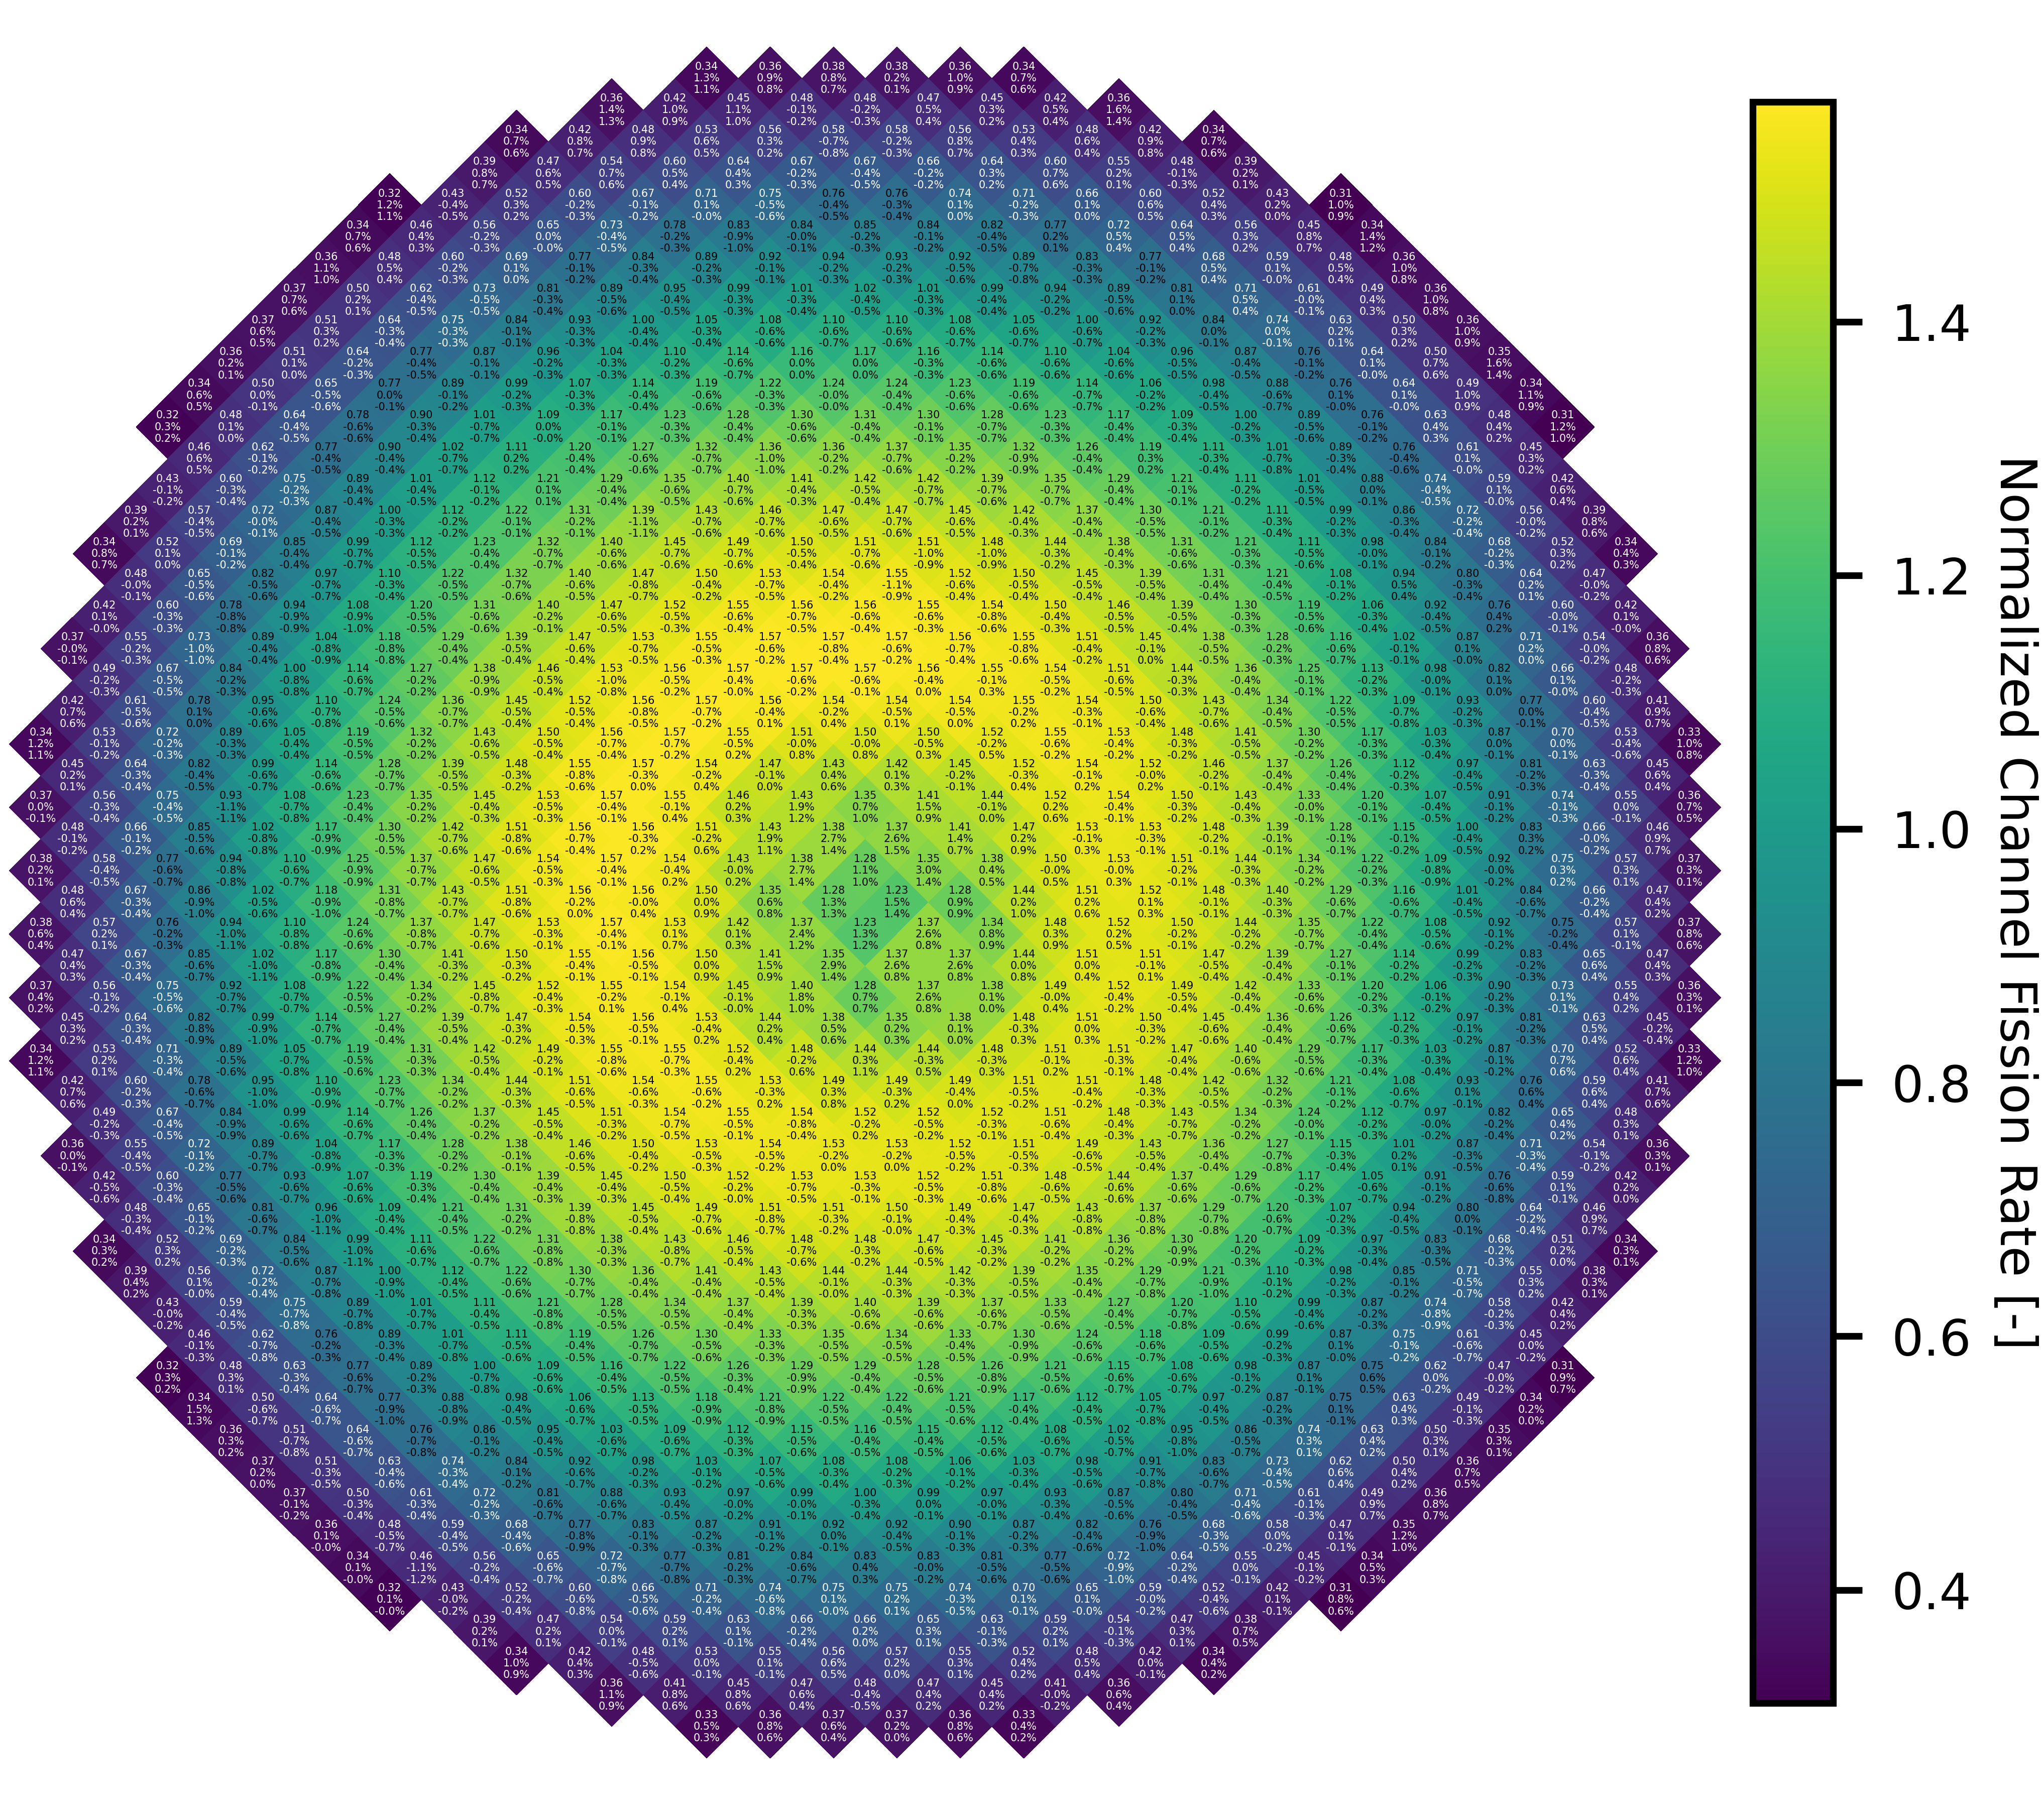
\includegraphics[width=\columnwidth]{msre-full-0-power}
  \caption{Normalized channel fission rate distribution of the 2-D \gls{MSRE} full-core model with
  no rod inserted.}
  \label{fig:0-rod}
\end{figure}

\begin{figure}[htb!]
  \centering
  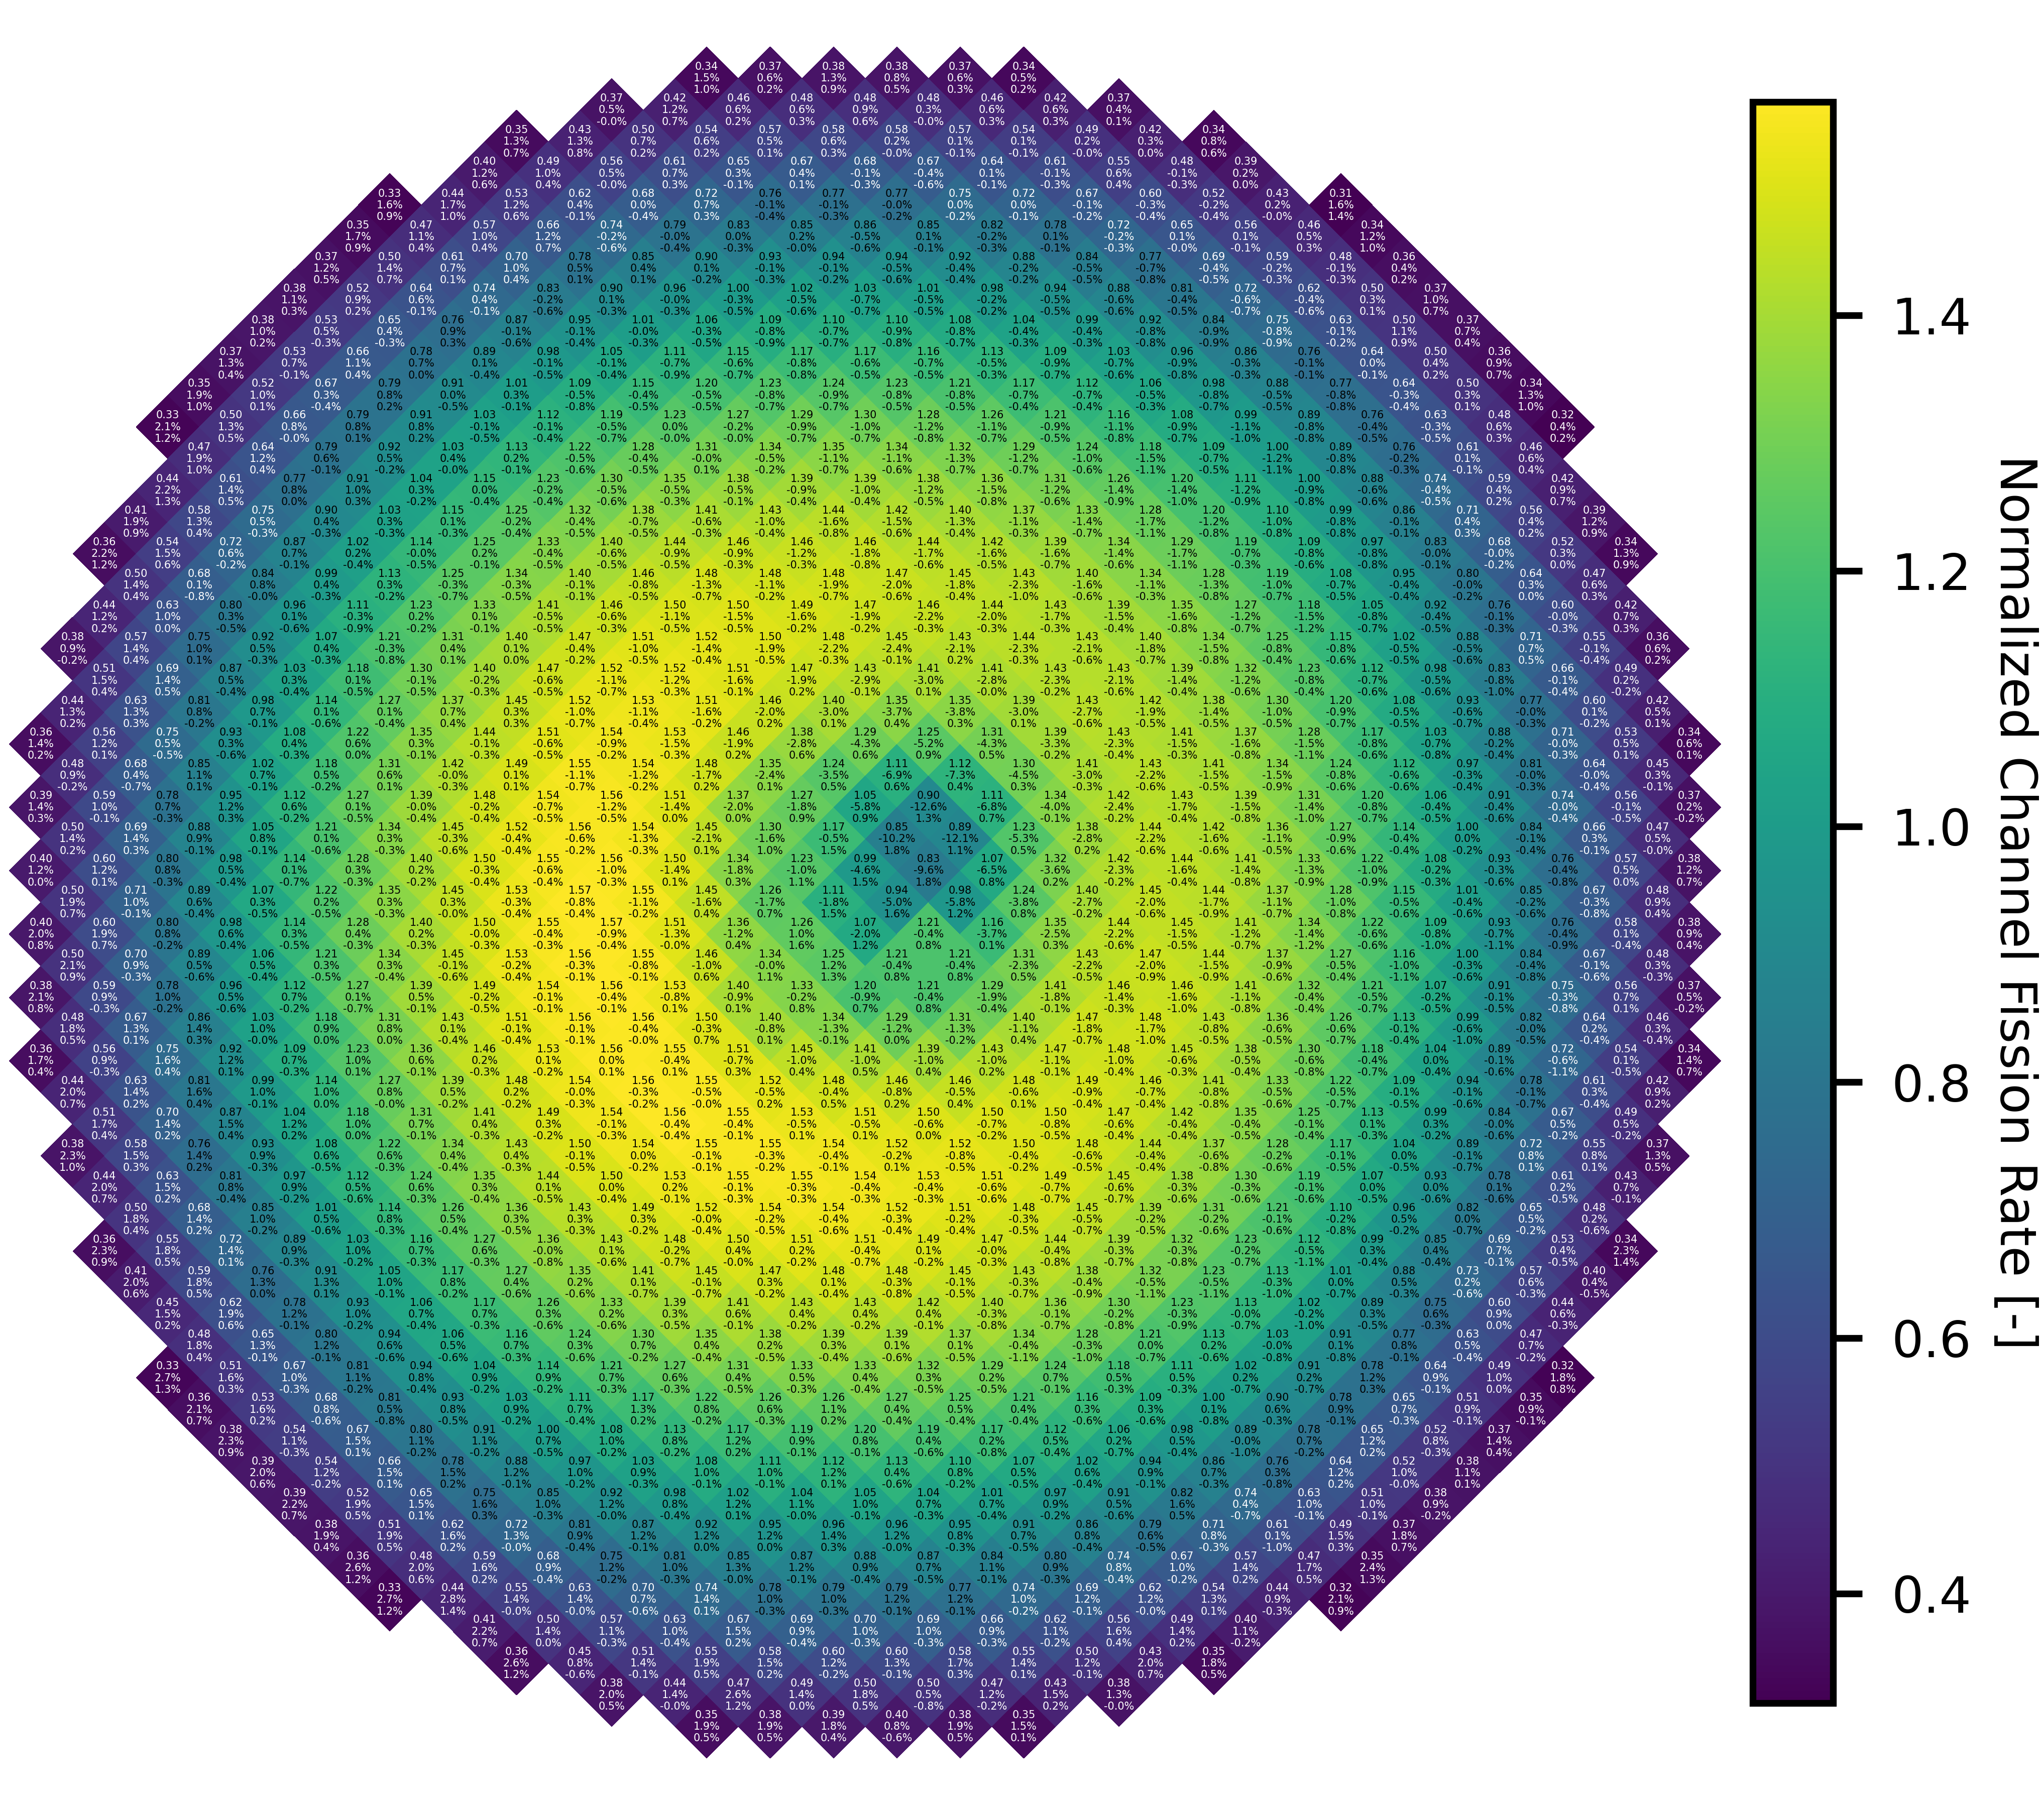
\includegraphics[width=\columnwidth]{msre-full-1-power}
  \caption{Normalized channel fission rate distribution of the 2-D \gls{MSRE} full-core model with
  Rod 1 inserted.}
  \label{fig:1-rod}
\end{figure}

\begin{figure}[htb!]
  \centering
  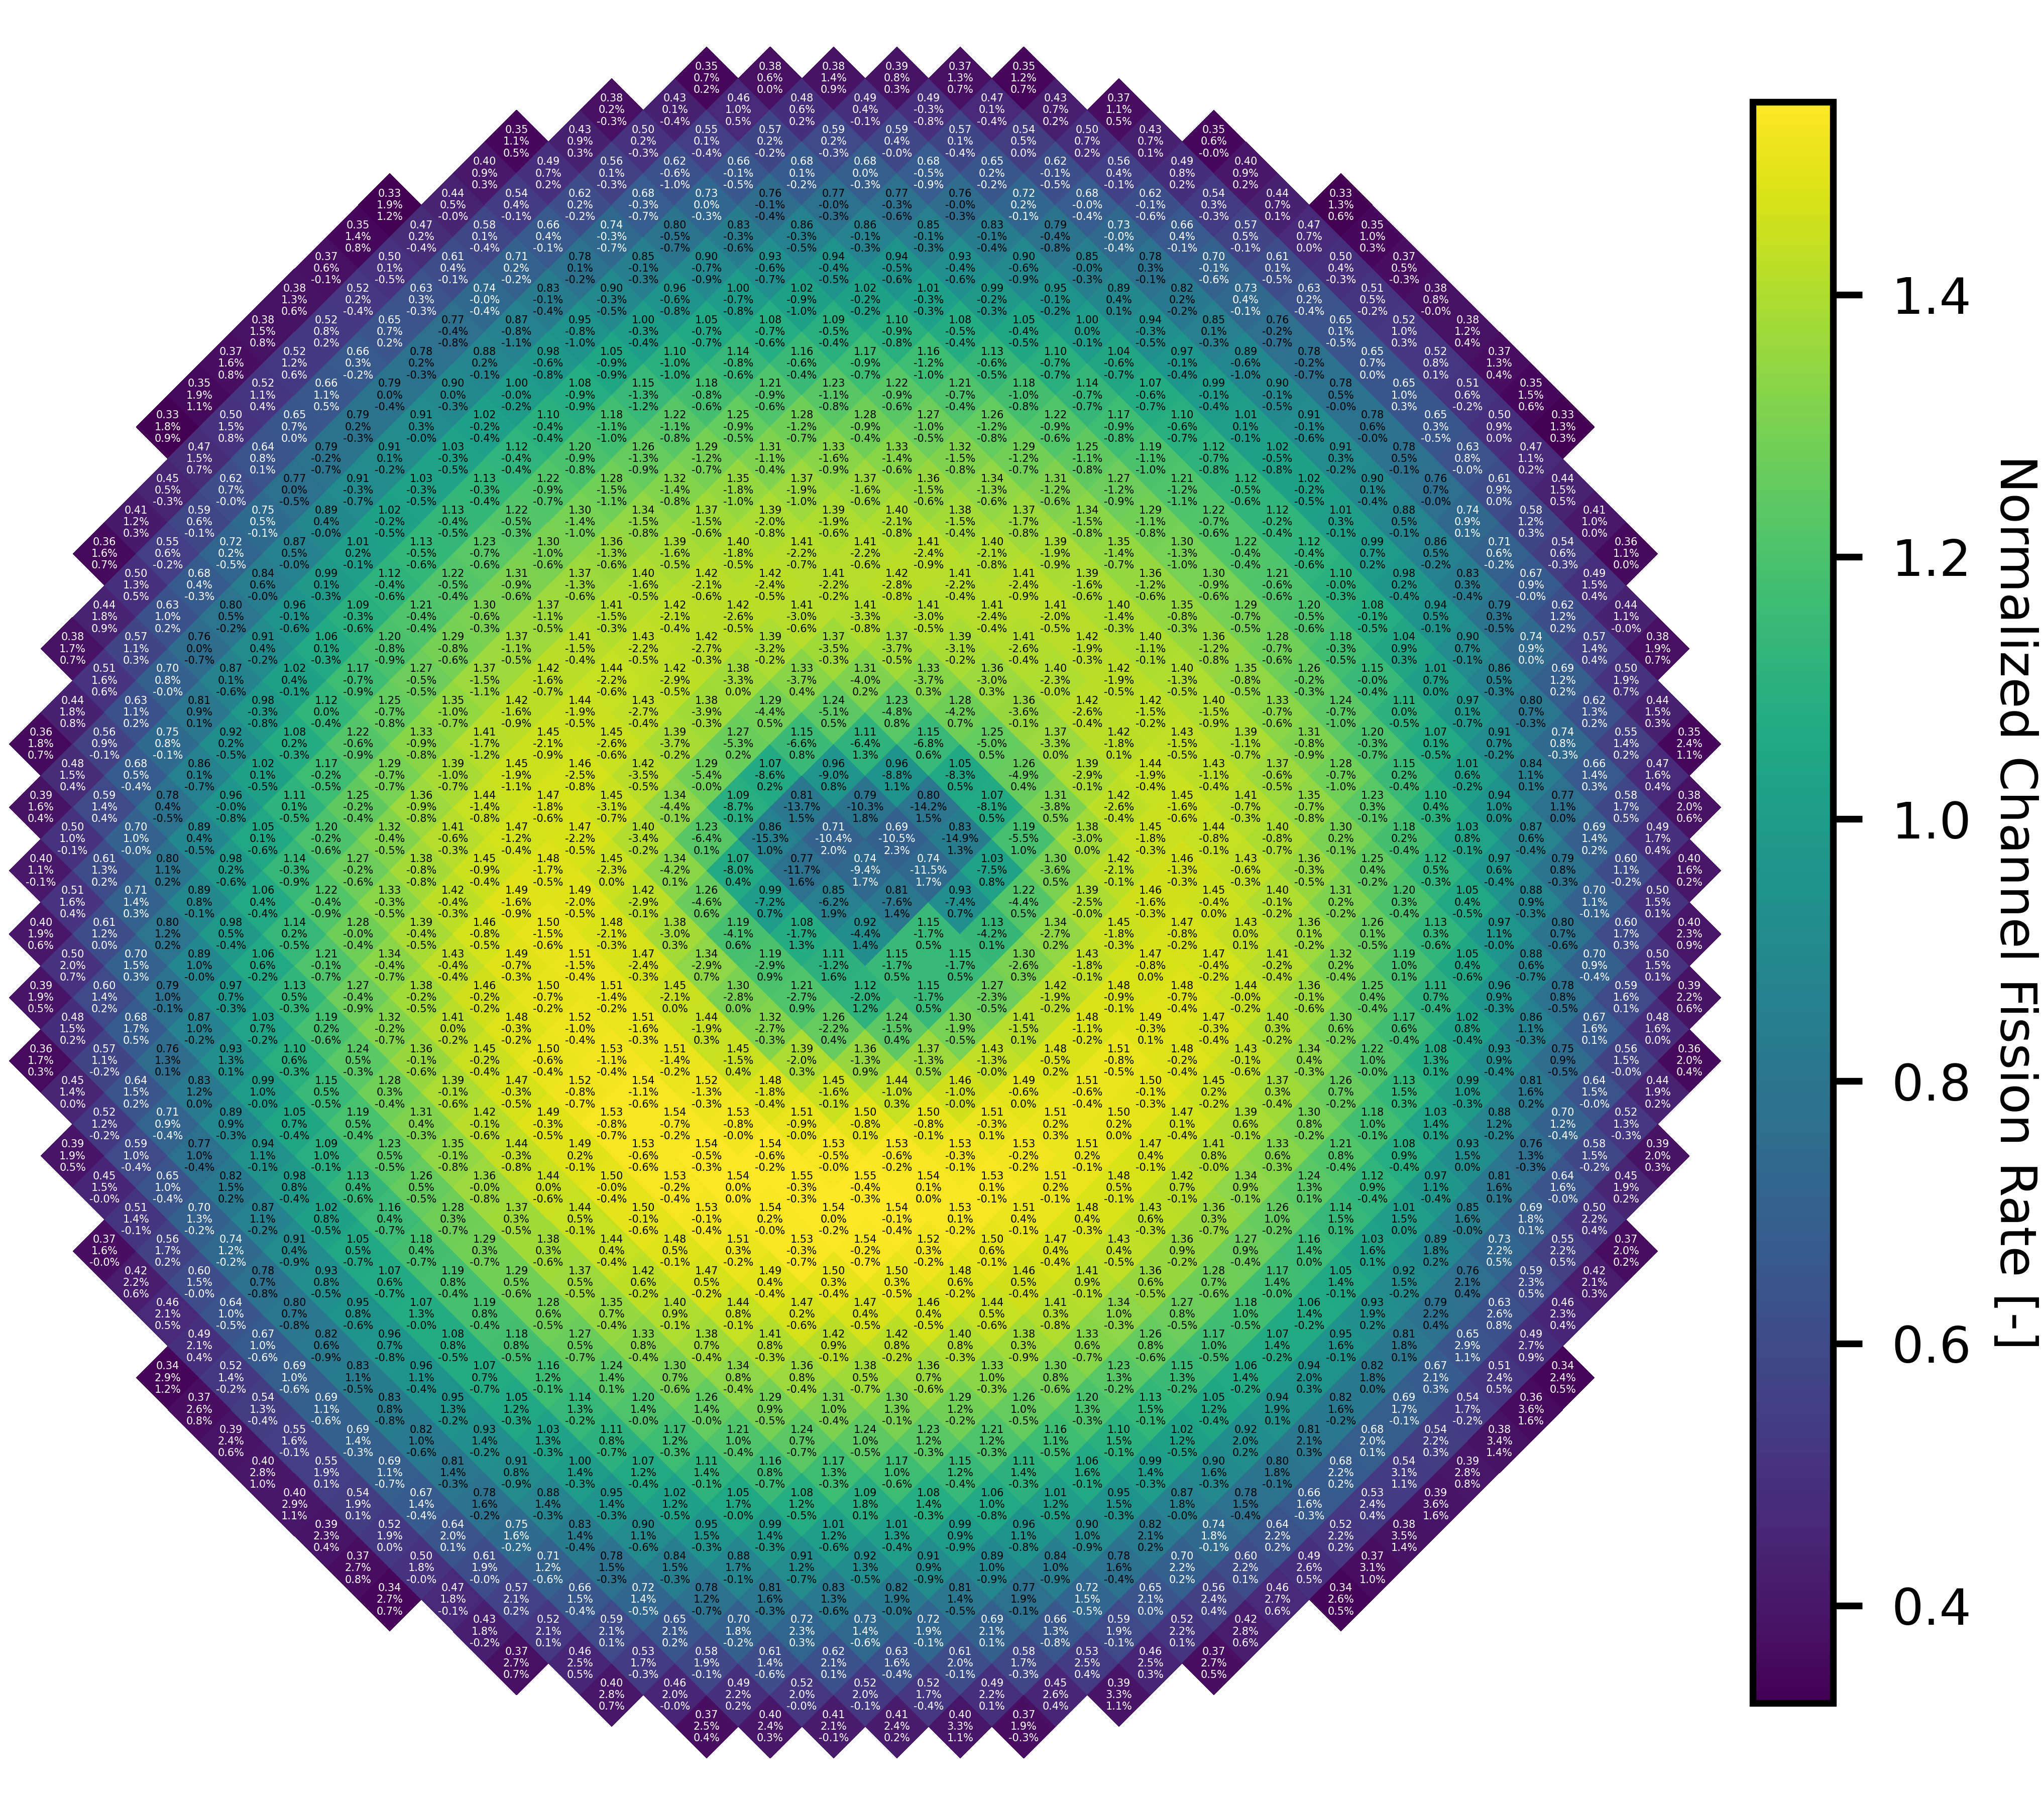
\includegraphics[width=\columnwidth]{msre-full-12-power}
  \caption{Normalized channel fission rate distribution of the 2-D \gls{MSRE} full-core model with
  Rods 1 \& 2 inserted.}
  \label{fig:12-rod}
\end{figure}

\begin{figure}[htb!]
  \centering
  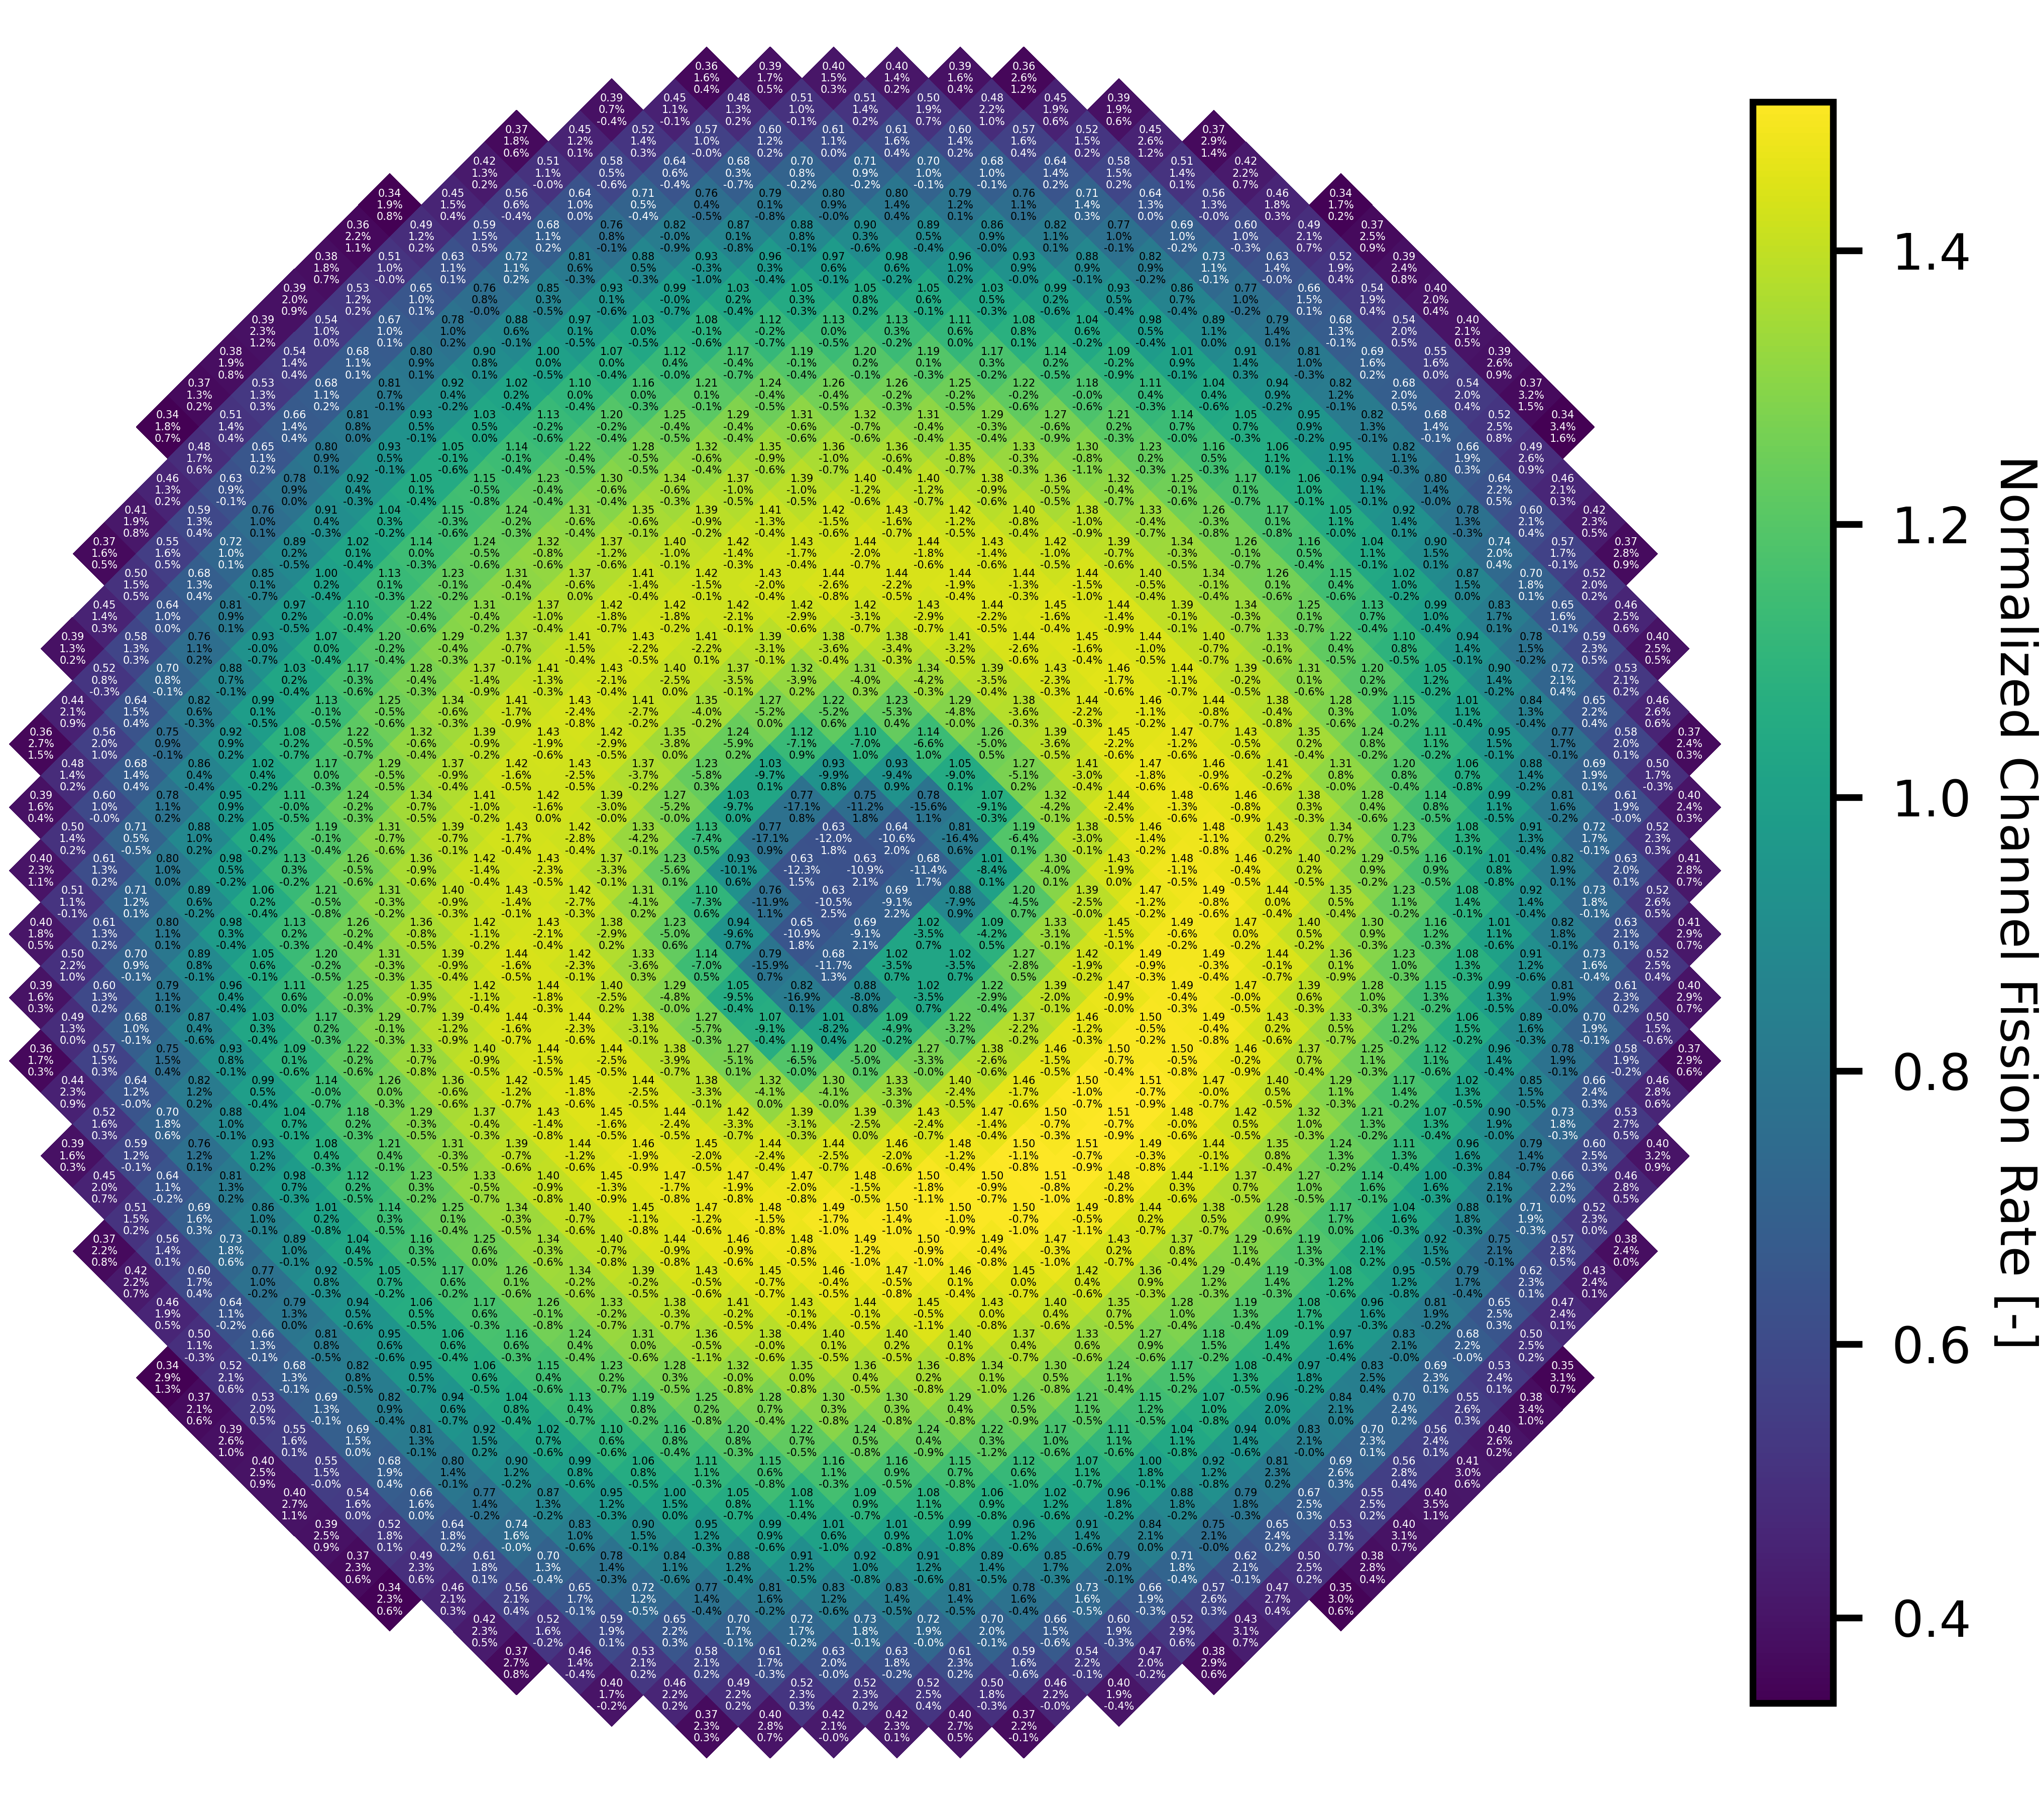
\includegraphics[width=\columnwidth]{msre-full-123-power}
  \caption{Normalized channel fission rate distribution of the 2-D \gls{MSRE} full-core model with
  Rods 1, 2 \& 3 inserted.}
  \label{fig:123-rod}
\end{figure}

